% project_proposal.tex
% CSC 4357 - Applied Computer Graphics - Dr. Robert Kooima

\documentclass[11pt,twocolumn]{article}
\usepackage[paperwidth=8.5in,paperheight=11in]{geometry}
\usepackage[cm]{fullpage}
\usepackage{titlesec}
\usepackage{graphicx}
\usepackage{hyperref}
\hypersetup{colorlinks=true,
	citecolor=blue}
\raggedbottom
\bibliographystyle{alpha}

% Section header titles to use small text
\titleformat*{\section}{\small\bfseries}

% Creating the title information
\title{From trivial fire simulation towards modern flames}
\author{Benjamin Guitreau\\
  \texttt{bguitr1@tigers.lsu.edu}}

\begin{document}
	% Displaying title
	\maketitle
	
	% Abstract
	\begin{abstract}
		This paper will propose the study of real-time simulations of fire and flames through the use of OpenGL and different mathematical and physics-based calculations to produce realistic models with typical flame behavior. Real-time simulations are beneficial to many industries and have the opportunity to save lives in given situations. Along with the practical uses, rendering realistic flames have an aesthetic value in the Film and Game industries.
	\end{abstract}
	
	% Introduction
	\section{Introduction}
		This project will serve as a learning tool for real-time simulation of fluids, mainly fire, using a novel flow-graph approach \cite{Zhang:2011:GFS:2019406.2019431} and a physics-based implementation \cite{Hong:2007:WFC:1276377.1276436} combined with the mathematics involved in chemical reactions. This project will also serve as a basis for artistic rendering using fire \cite{Bangalore:2012:TAD:2328888.2328896}.
		
	% Related work
	\section{Relevance}
	The simulation of real-time events is extremely difficult and improbable in most situations; however, with the capabilities of modern computers and super-computers, these simulations can be handled with computer graphics. By generating a flame or fire that behaves realistically could be used in a building simulation to help engineers refine the structural design and to allow safety personnel a better viewpoint that allows for updating protocols and policies. Another application for fire simulations is a forest fire simulation that could give advance notice to residents and possibly allow for firefighters to preemptively strike where the forest fire will direct its energies next. Hollywood also benefits from better fire simulations. Movies such as "How to Train Your Dragon" give ample examples of how computer graphics can be used to bolster and enhance animations and traditional film \cite{Robertson:2010:TE}.
	
	% Procedures
	\section{Procedure}
	The project will begin with the researching of a flame rendered with a basic texture. From this vantage point, the project will have a basis to which all comparisons of difficulty in coding, computational costs, and performance costs of animations will be allowed to be processed and analyzed. The second phase will consist of adding animation to the fire and calculating fuel sources that will either be extinguished as the fire burns out or have yet to catch on fire. The third phase will be in the research and implementation of flames rendered using Navier-Stokes equations and detonating shock dynamics(DSD) \cite{Hong:2007:WFC:1276377.1276436}. This process will also bring into use PhysBAM from Stanford University \cite{Dubey:2011:PPB:2037636.2037646}. PhysBAM is a simulation library developed at Stanford University and is used in the academic world and by industry members including but not limited to Disney Animation and Pixar Animation Studios \cite{Dubey:2011:PPB:2037636.2037646}. The fourth phase will be to research a flow-graph method that uses less computational resources than the previous Navier-Stokes method \cite{Zhang:2011:GFS:2019406.2019431}. Zhang et al. describes using a data-driven method for synthesizing fire animations at a much lower computation cost. \cite{Zhang:2011:GFS:2019406.2019431} The fifth phase is more oriented towards the Arts and as such will be based upon generating flames in such a visual manner that they are shaped into a natural object, such as a lion or wolf. \cite{Bangalore:2012:TAD:2328888.2328896} The final phase of the project will be the analysis of all gathered data, objective and subjective, and present the final renderings of each phase.
	
	% Conclusion
	\section{Conclusion}
	The project will play an integral part in future research areas and will embellish upon my studies of OpenGL and visualizations.
	
	% Start a new page for the images and flush any floats
	\clearpage
	
	% Figure 1 taken from Wrinkled Flames and Cellular Patterns
	\begin{figure}[h!]
		\caption{A dragon emits a flame.}
		\label{dragon_full}
		\centering
				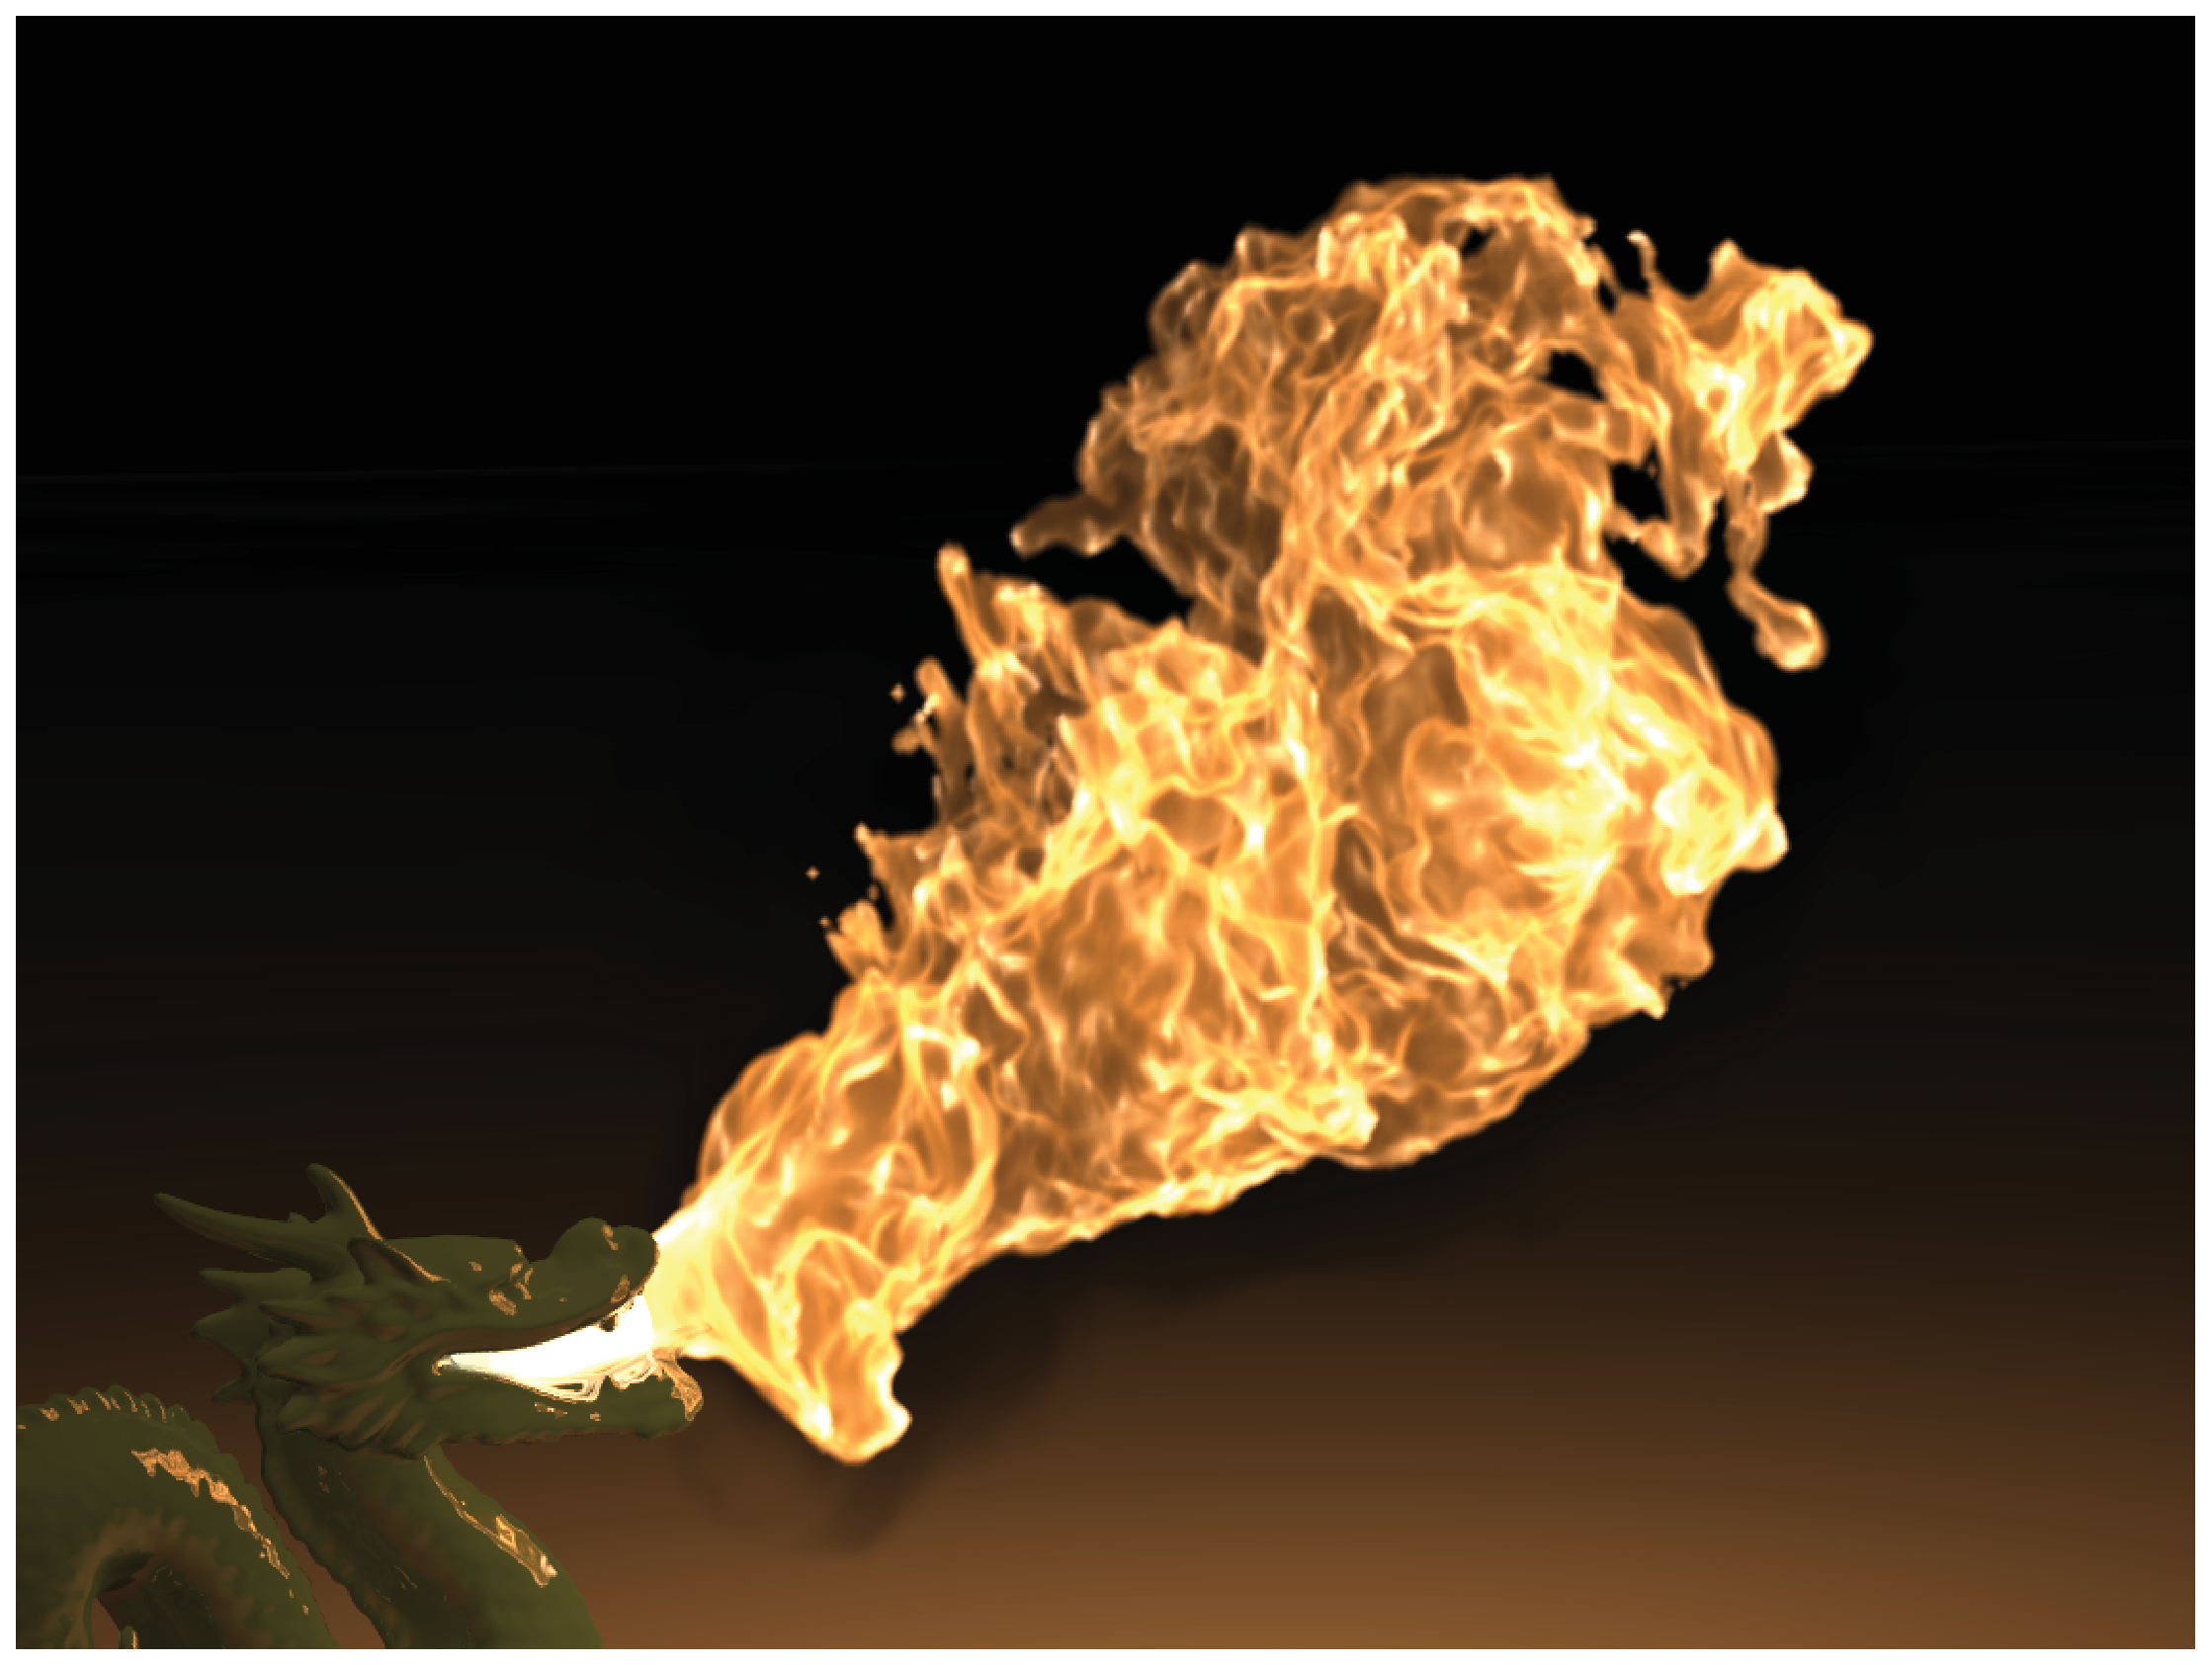
\includegraphics[height=2.5in]{dragon_full.eps}
	\end{figure}
	% Figure 2 taken from Graph-Based Fire Synthesis
	\begin{figure}[h!]
		\caption{A fire synthesized using a flow-graph method with visually plausible transitions}
		\label{firewall}
		\centering
			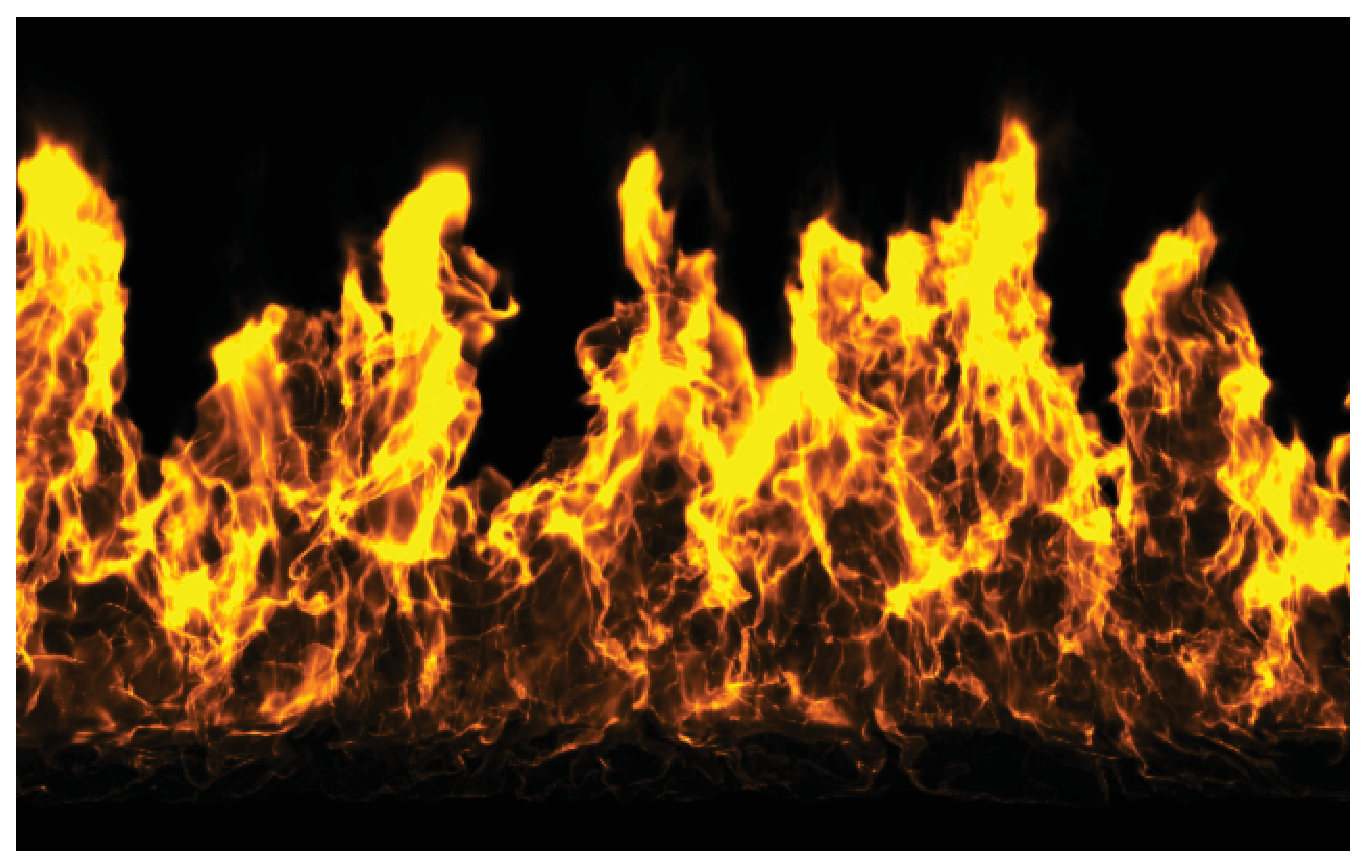
\includegraphics[height=2.5in,width=2.5in]{firewall.eps}
	\end{figure}
	% Figure 3 taken from A Technique for Art Direction of Physically Based Fire Simulation
	\begin{figure}[h!]
		\caption{A wolf shaped flame.}
		\label{wolf}
		\centering
			
\includegraphics[height=2.5in]{wolf.eps}
	\end{figure}
	
	\pagebreak
	
	% Figure 4 taken from Wrinkled Flames and Cellular Patterns
	\begin{figure}[h!]
		\caption{A dragon's flame after emission.}
		\label{dragon_puff}
	 	\centering
	 		\includegraphics[height=2.5in]{dragon_puff.eps}
	\end{figure}
	% Figure 5 taken from Graph-Based Fire Synthesis
	\begin{figure}[h!]
		\caption{A vertical pillar of fire using a flow-graph method with visually plausible transitions.}
		\label{firecone}
		\centering
			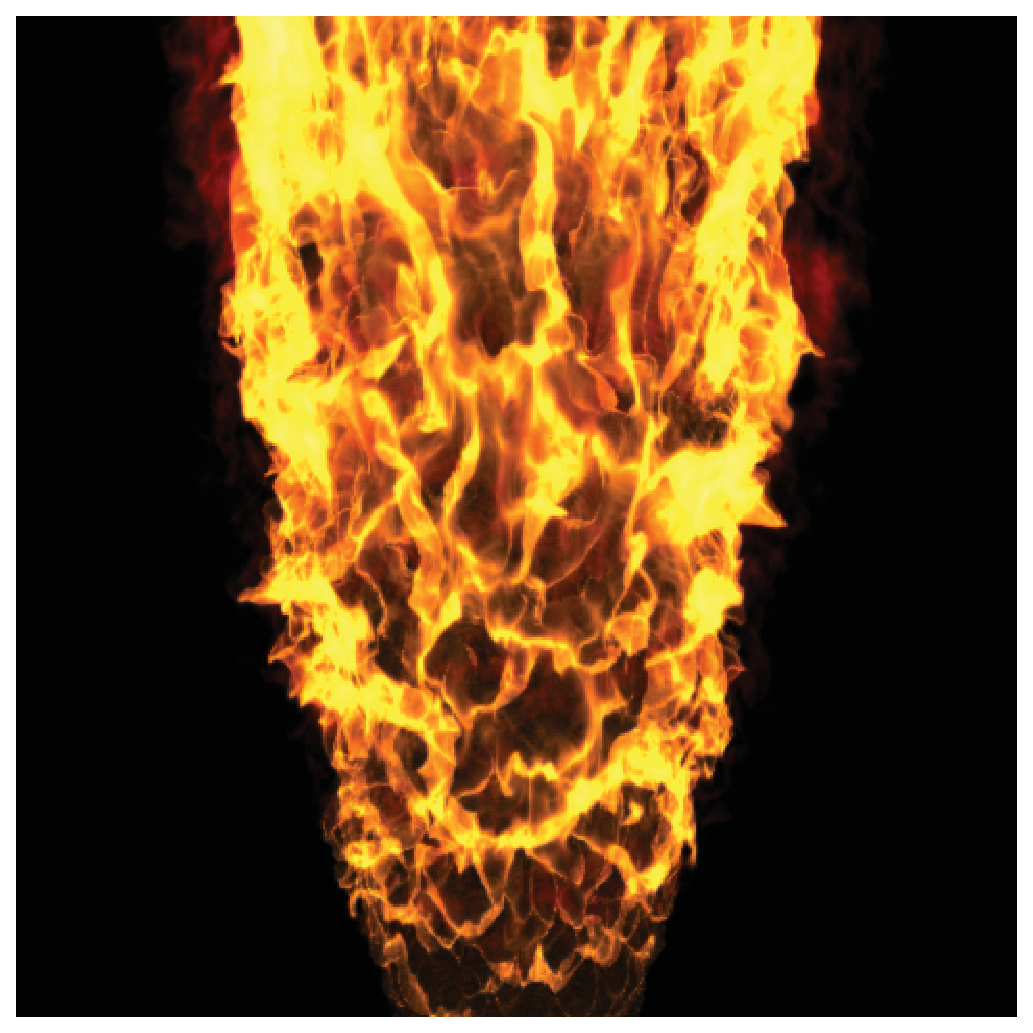
\includegraphics[height=2.5in]{firecone.eps}
	\end{figure}
	% Figure 6 taken from A Technique for Art Direction of Physically Based Fire Simulation
	\begin{figure}[h!]
		\caption{A lion shaped flame.}
		\label{lion}
		\centering
			
\includegraphics[height=2.5in]{lion.eps}
	\end{figure}
	
	% Start a new page for the bibliography and flush any floats
	\clearpage
	
	% Load references
	\bibliography{project_proposal}
\end{document}